\documentclass{article}

\usepackage[a4paper, total={6in, 8in}]{geometry} % Page margins
\usepackage[utf8]{inputenc}
\usepackage{amsmath, amssymb, mathtools, amsfonts, amsthm}
\usepackage{wasysym} % Smiley QED
\usepackage{eulervm} % Font
\usepackage{fancyhdr} % Custom headers and footers
\fancyhead[C]{\thepage} % Page numbering for center header
\usepackage{mdframed}
\usepackage{xcolor}
% list environments               
\usepackage{enumerate}            
\usepackage[shortlabels]{enumitem}      

% Code block environment
\usepackage{listings}            
\lstset{basicstyle = \ttfamily, mathescape}



% figure support
\usepackage{tikz}
\usepackage{graphicx}
\usepackage{import}
\usepackage{xifthen}
\pdfminorversion=7
\usepackage{pdfpages}
\usepackage{transparent}

\pdfsuppresswarningpagegroup=1
\title{DSA: Exercise 3}
\author{David Sermoneta}
\begin{document}
\maketitle
\section*{Exercise 1:}
\subsection*{Exercise 1.a)}
\begin{lstlisting}[numbers = left]
  : 5 9
  : 5
  : 9
  : LR 5 9
  : 3 8 2
  : 3
  : 8 2
  : 8
  : 2
  : LR 8 2
  : LR 3 8
  : LR 9 8 
\end{lstlisting}

\subsection*{Exercise 1.b)}
Since we call the function twice, that sets $a = 2$, and each call halves $n$ by 2,
this gives us $b=2$. Further, we have $3$ \texttt{PRINT} statements, as well
as 2 operations that take constant time, thus $d = 0$. We get the following form: \[
T(n) = 2T\left(\left\lfloor \frac{n}{2} \right\rfloor \right) + 5\Theta(1) .
\] Since $2 > 2^{0}$, we have that  \[
T(n) = \Theta(n^{\log_b(a)}) = \Theta(n),
\] and we are done.


\subsection*{Exercise 1.c)}
Apart from the obvious: getting rid of the print statements, there isn't anything
else to do. We can explain this via the following reasoning. apart from the 
print statements, there are: 
\begin{enumerate}
    \item Base case of the recursion formula,
    \item initializing of the variable $k$ that is used in the rest of the code,
    \item calling the function on the sliced list \texttt{A[1 : k} and  \texttt{
        A[k : A.length]}.
\end{enumerate}
Removing any of these, would result either in the function not 
ending, a code error, or a function that 
does not find the maximum of a list, but rather, a shorter version of the list.
So the answer is, one can only remove the three print stamements to have the
algorithm still find the maximum element of a given array.

\section*{Exercise 2:}

\begin{figure}[htpb]
    \centering
 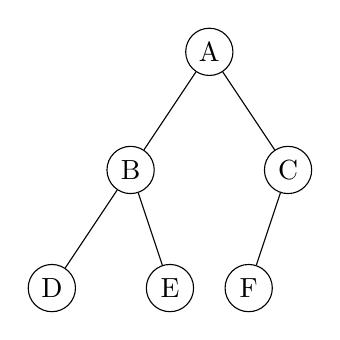
\begin{tikzpicture}[every node/.style={circle, draw, inner sep=2pt, minimum size=6mm}]
     \node (A) at (0,0) {A};
     \node (B) at (-1,-1.5) {B};
     \node (C) at (1,-1.5) {C};
     \node (D) at (-2,-3) {D};
     \node (E) at (-0.5,-3) {E};
     \node (F) at (0.5,-3) {F};
      
     \draw (A) -- (B);
     \draw (A) -- (C);
     \draw (B) -- (D);
     \draw (B) -- (E);
     \draw (C) -- (F);
 \end{tikzpicture}
 \caption{Graph with both inorder and preorder traversal}
\end{figure}
\begin{figure}[htpb]
    \centering
\begin{tikzpicture}[every node/.style={circle, draw, inner sep=2pt, minimum size=6mm}]     
   \node (A) at (0,0) {A};
    \node (B) at (-1,-1.5) {B};
    \node (C) at (-4,-6) {C};
    \node (D) at (-2,-3) {D};
    \node (E) at (-3,-4.5) {E};
    \node (F) at (-5,-7.5) {F};
                 
    \draw (A) -- (B);
    \draw (B) -- (D);
    \draw (D) -- (E);                                                                                                    
    \draw (E) -- (C);
    \draw (C) -- (F);
\end{tikzpicture}
\caption{Graph with only preorder traversal specified, it is not the same as
the one in figure 1, so the preorder traversal does not determine $T$ uniquely.}
\end{figure}
\section*{Exercise 3:}
For graph ($i$), we have height($T_{i}$) = $3$, depth($3$) = $2$, and it neither
FB, NC nor C. \\
For graph ($ii$), we have height($T_{ii}$) = $3$, depth($3$) = $1$, and it is all of
the above.  \\
For graph ($iii$), we have height($T_{iii}$) = $2$, depth($3$) = $2$, and it is
only NC.  \\
For graph ($iv$), we have height($T_{iv}$) = $2$, depth($3$) = $0$, and it is only
FB. 
\section*{Exercise 4:}
\begin{lstlisting}[numbers = left]      
MERGESORT(A,1,3) 
MERGESORT(A,1,2) 
MERGESORT(A,1,1) 
MERGESORT(A,2,2) 
MERGE(A,1,1,2) $\to$ [2,6]
MERGESORT(A,3,3)
MERGE(A,1,2,3) $\to$ [2,3,6]
\end{lstlisting}
\end{document}
